\chapter{Definición del problema}
\label{sect:problemdefinition}

Definiremos aquí el problema formalmente como uno de programación matemática. Sea una red que modela una ciudad, denotada por un grafo dirigido $G=(N,A)$, compuesto por el conjunto de vértices $N$ y el conjunto de arcos $A$. El grafo representa la red subyacente donde pueden ser construidas infraestructuras de ciclovías por ejemplo la red de calles de una ciudad o una simplificación de ella. Cada arco $a \in A$ está ponderado por su largo $l_a$. Un conjunto de pares origen-destino $OD \subseteq N^2$, y su demanda asociada $D = \{d_k,\; k \in OD\}$ donde cada valor $d_k$ es la cantidad de viajes que potencialmente podrían ser en bicicleta para un horizonte de tiempo fijo, por ejemplo en un día. Y funciones $f_k,\;k \in OD$ que determinan la cantidad de la demanda de cada par origen-destino que utiliza la bicicleta en función del costo de usuario de ir desde su origen $O(k) \in N$ hasta su destino $S(k) \in N$. El objetivo es maximizar la cantidad de demanda que utiliza la bicicleta como modo de transporte. Para poder lograr esto se cuenta con diferentes tecnologías de ciclovías y un presupuesto, que de ser utilizados permiten disminuir el costo percibido por los usuarios al utilizar la bicicleta y por lo tanto potencialmente influir en la decisión de utilizarla como modo de transporte. Asumimos que todos los usuarios utilizan el camino más corto para trasladarse entre dos puntos y que sus decisiones respecto a qué medio de transporte utilizar puede variar según lo modela las funciones de transferencia de demanda.

Partimos de una formulación matemática binivel del problema ya que nos da una representación directa y clara de lo que queremos resolver. Este tipo de problema se estructura definiendo dos entidades jerárquicas en diferentes niveles que representan intereses (u objetivos) no necesariamente alineados \citep{bardbook}. En nuestra formulación, el primer nivel representa la comuna (o entidad que toma decisiones sobre las ciclovías) y busca maximizar la cantidad de usuarios que utilizan la bicicleta por medio de la decisión de la ubicación y tipo de ciclovías a utilizar en cada arco de la red. El segundo nivel representa a los usuarios y busca minimizar el costo del camino más corto para cada par origen-destino. Existe interacción en ambos sentidos de la jerarquía, mientras el nivel inferior depende de las decisiones del nivel superior para calcular los caminos más cortos, el nivel superior depende de los costos de los caminos más cortos para calcular la demanda que se transfiere.

Analizaremos los problemas por separado y luego relacionados para ver cómo el planteo binivel expresa adecuadamente nuestro problema. En primer lugar discutiremos algunas consideraciones respecto a lo que esperamos como salida, o de otra forma, lo que nos interesa obtener de la resolución. Viendo exclusivamente el objetivo, podemos decir que este planteo binivel es un modelo que nos dice cuánta demanda se puede atraer a la bicicleta como medio de transporte dado un presupuesto y la realidad de una ciudad (datos de red y matriz de demanda). Esto tiene sentido por sí mismo, ya que permite tomar decisiones fundadas sobre qué presupuesto tiene sentido asignar a la construcción de ciclovías en dicha ciudad. Sin embargo, el valor de demanda que se transfiere a la bicicleta no es independiente de las decisiones de dónde y cuáles tecnologías de ciclovía construir. Éstas decisiones también son de nuestro interés por se la solución que lleva al valor óptimo que luego podemos analizar y representar gráficamente.

La formulación que planteamos considera aspectos de modelos descriptivos en donde el objetivo es simular el comportamiento de los usuarios, en nuestro caso obtener el recorrido de los usuarios y su costo dado un estado de la red de ciclovías; y modelos normativos en donde el objetivo es mejorar las decisiones que afectan un proceso, es decir cómo mejorar o planificar la red de ciclovías para atraer más ciclistas. Mezclar ambos puede resultar en modelados complejos, el modelado del comportamiento de los usuarios ya es un problema de optimización entonces al agregar decisiones de otro actor debemos agregar variables de decisión, restricciones y eventualmente otro objetivo lo que puede llevar a una estructura no lineal, binivel o de múltiples objetivos.

El problema de segundo nivel es el clásico problema de encontrar el costo del camino más corto entre un par de nodos en un grafo ponderado. Puede ser formulado como un problema de flujo de costo mínimo y por lo tanto resoluble eficientemente con el algorítmo Simplex o método de punto interior en tiempo polinomial obteniendo flujos unitarios \citep{networkflowsbook}. A su vez existen algorítmos específicos que también resuelven el problema de forma exacta eficientemente \footnote{Ejemplo: Dijkstra, Bellman-Ford, Formulación LP de flujo de costo mínimo y otros.}. En nuestro caso tenemos $|OD|$ problemas independientes del camino más corto puesto que no consideramos restricciones de capacidad en los arcos ni efectos de la congestión \citep{Sheffi1985}. Estos problemas independientes pueden ser modelados en una única formulación de flujos de costo mínimo. Modelamos de esta forma el comportamiento de los usuarios que en general que nos trasladamos por los caminos más cortos según nuestro entendimiento, según cierta magnitud objetiva, entre un par de puntos. En este sentido, en \cite{winters2010} se menciona que los ciclistas en general no se trasladan por el camino más corto en distancia sino que realizan desvíos para circular por vías mas favorables para la bicicleta. Decimos entonces que los usuarios se trasladan por el camino más corto según una magnitud que involucra en su estimación la distancia y el tipo de vía que se utilice.

El problema de primer nivel es el que interrelaciona a los $|OD|$ problemas del costo del camino más corto. Por ejemplo, decidir construir una tecnología de ciclovías en un arco puede afectar el costo del camino más corto para varios pares origen-destino. Por otro lado, puede pensarse que decidir dónde construir ciclovías está ligado al recorrido de los caminos más cortos sobre la red previo a la construcción de ciclovías, pero como se muestra en el siguiente ejemplo esto no necesariamente es así. Este problema tampoco es independiente del recorrido de los caminos más cortos, sin embargo, estos recorridos deberían computarse una vez decididas las infraestructuras a construir, y esta es la dificultad inherente del problema en su totlidad, dado que no es posible determinar qué decisiones inducen los mejores caminos.

\section{Hipótesis}

En este trabajo asumimos las siguientes hipótesis que entendemos tienen sentido en este contexto:

\begin{itemize}
  \item{El tiempo de viaje en todo arco de la red es independiente del flujo sobre el mismo. En general el modelado del tráfico en bicicleta no considera capacidades ni congestión por los valores de demanda y flujo que se manejan \citep{Sheffi1985}. La literatura sobre redes de ciclovía estudiada también asume esta hipótesis \cite{Lin2013}, \cite{Duthie2014} y \cite{Liu2019}, \cite{Zhu2019} y \cite{baya2021}. Además de ser uno de los resultados del análisis en \cite{broach2012} para la ciudad de Portland, Estados Unidos. Por otro lado, tras una encuesta realizada en Copenhague, Dinamarca, donde se realizan un 35\% de los viajes en bicicleta, se deduce que las congestión de bicicletas tiene un impacto negativo en las preferencias de los ciclistas que están dispuestos a desviarse de sus caminos más cortos para evitar esta situación \citep{Vedel2017}. Sin embargo reconocen que otras ciudades lejos de llegar a esta situación.}
  \item{Existen diferentes pares origen-destino en la red, cada uno con un valor de demanda. Para cada par existe al menos un camino sobre el grafo $G$ que une el origen y el destino.}
  \item{Los usuarios siempre buscan minimizar el costo de su viaje (todos son perfectos optimizadores y se comportan igual).}
\end{itemize}

Sobre la red, consideramos que los grafos son dirigidos y cuando se decide construir infraestructura de ciclovía sobre un arco solo se hace en la dirección del mismo. Esto simplifica el modelado y le da mayor flexibilidad. Con esta simplificación no estamos teniendo en cuenta que el costo marginal de construir una ciclovía en un sentido, dado que existe la misma infraestructura en el otro sentido, puede ser menor al costo de construir la primera. Tampoco restringimos que en una solución, dados dos nodos mutuamente adyacentes, se decida construir diferentes tecnologías en cada sentido.

\section{Características de una solución}
\label{sect:solutioncharacteristics}

Como marco para para evaluar la validez del modelo definimos algunas características deseables que, entendemos, deben cumplir una solución del problema.

Consideramos que una solución cumple las siguientes propiedades:

\begin{enumerate}
    \item{El costo de los caminos más cortos entre pares origen-destino sobre la red resultante, es decir, adicionando ciclovías, es menor o igual al costo sobre la red sin ciclovías.}
  \item{\label{budgetexcess} El presupuesto excedente no es suficiente para agregar infraestructura que mejore el costo de alguno de los caminos más cortos.}
  \item{El camino más corto sobre la red resultante para un par origen-destino no puede inducir un valor de demanda transferida distinto al de la solución.}
\end{enumerate}

\section{Ejemplo - Aplicación de modelo binivel}
\label{sect:example1}

Consideramos una instancia del problema y su solución óptima para mostrar cómo el planteo binivel modela correctamente el problema que queremos resolver y cómo la solución óptima cumple con las condiciones de este planteo. Veremos que la solución es óptima en el sentido que induce la mayor cantidad de demanda transferida posible.

Sea la red modelada por el grafo de la Figura \ref{fig:example1base}, donde tenemos dos pares origen-destino (1, 5) y (2, 6) cada uno con una demanda de magnitud $D$, un presupuesto de 11 unidades, dos tipos de tecnologías de ciclovías: la base (tecnología 0 o red de calles) y la tecnología 1. Consideramos que los arcos tienen un largo asociado y para la tecnología base el costo de construcción es 0, al ser esta la red de calles y que el costo de usuario es igual al largo del arco. Para la tecnología 1 el costo de construcción es igual al largo del arco y el costo de usuario es la mitad que el de la tecnología base, ver Tabla \ref{table:example1arccosts}. Finalmente, la transferencia de demanda para ambos pares origen-destino está modelada por la función $f$ que dado un valor del costo de usuario de un camino devuelve una cantidad de demanda que cambia de modo de transporte a la bicicleta:

$$
  f(x) = \left\{ \begin{array}{lcr}
          D & \mbox{si}   & x < 4 \\
          0 & \mbox{sino} &
  \end{array}
  \right.
$$

\begin{table}[h!]
  \centering
  \begin{tabular}{cccccc}
    \toprule
    Arco & CU base & CU 1 & CC base & CC 1 & \\
    \midrule
      (1, 3) & 2 & 1   & 0 & 2 \\
      (1, 5) & 6 & 3   & 0 & 6 \\
      (2, 3) & 2 & 1   & 0 & 2 \\
      (2, 6) & 6 & 3   & 0 & 6 \\
      (3, 4) & 3 & 1,5 & 0 & 3 \\
      (4, 5) & 2 & 1   & 0 & 2 \\
      (4, 6) & 2 & 1   & 0 & 2 \\
    \bottomrule
  \end{tabular}
    \caption{Resumen de costos de usuario (CU) y de construcción (CC) para cada tecnología de ciclovía.}\label{table:example1arccosts}
\end{table}

\begin{figure}[h!]
  \centering
  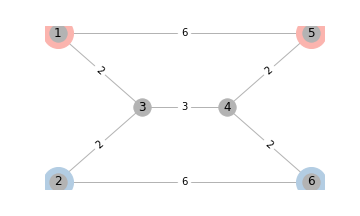
\includegraphics[width=6cm]{../resources/example_1_base.png}
  \caption{Representación de la red utilizada para el ejemplo de aplicación de la formulación binivel. Los dos pares origen-destino se detallan con un color diferente. Cada arco tiene una etiqueta con el costo de usuario sobre la tecnología base, es decir, la red de calles.}
  \label{fig:example1base}
\end{figure}

Podemos deducir rápidamente de la Figura que representa la red \ref{fig:example1base}, que el camino más corto para ambos pares origen-destino sobre la red de calles está compuesto por un solo arco de costo 6. El objetivo entonces es decidir dónde construir tecnología 1 tal que el costo de los caminos más cortos de uno o ambos pares origen-destino sea menor a 4 unidades (dada la función de transferencia de demanda), de manera que una cantidad $D$ o $2D$ de demanda total pueda ser transferida a la bicicleta. Nótese que los valores posibles de demanda transferida total en este caso solo pueden ser $0$, $D$ y $2D$. Si decidimos utilizar tecnología 1 en alguno de los arcos (1, 5) o (2, 6), digamos el primero, entonces nos aseguramos que la demanda del par origen-destino (1, 5) será transferida a la bicicleta, ya que el costo del camino más corto pasa a ser $3$. Con el presupuesto remanente de valor $5$, solo podremos construir tecnología 1 en a lo sumo dos de los arcos (2, 3), (3, 4) y (4, 6). No es difícil ver que a lo sumo podremos mejorar el costo del camino más corto a $4.5$ para el par origen-destino (2, 6). La demanda transferida total en este caso es entonces de $D$.

La solución óptima viene de construir tecnología 1 en todos los arcos del grafo menos los (1, 5) y (2, 6). Esto permite que ambos pares origen-destino tengan un nuevo recorrido como camino más corto, de costo $3.5$, lo que permite, según la función de transferencia de demanda, transferir $2D$ unidades de demanda. Esta solución se puede observar gráficamente en la Figura \ref{fig:example1solution}.

\begin{figure}[h!]
  \centering
  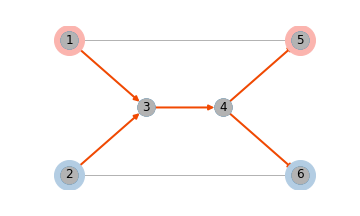
\includegraphics[width=6cm]{../resources/example_1_infras.png}
  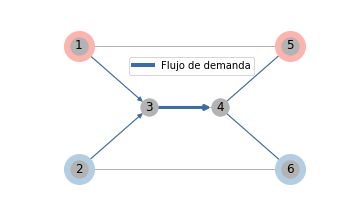
\includegraphics[width=6cm]{../resources/example_1_flows.png}
  \caption{Representación de la solución óptima en el grafo. A la izquierda se muestra en naranja en cuáles arcos se construye la tecnología 1. A la derecha, en azul, los flujos sobre los caminos más cortos para ambos pares origen-destino. Nótese que el ancho del arco en este caso da una noción de la cantidad flujo.}
  \label{fig:example1solution}
\end{figure}

\FloatBarrier
\section{Formulación matemática de dos niveles}

Presentamos la formulación matemática formal. Sean:

\begin{description}
  \item[$I$]: Conjunto índice de tipos de tecnologías de ciclovías, numeradas desde $0$ en adelante. A mayor valor del índice mejor es la tecnología para el usuario, es decir tiene menor costo de usuario, y mayor el costo de construcción. El indice 0 corresponde a la calle y representa la no construcción de infraestructura de ciclovía.
  \item[$C_{ai}$]: Costo de usuario de atravesar el arco $a \in A$ utilizando la tecnología $i \in I$. $C_{ai} > 0$.
  \item[$H_{ai}$]: Costo de construcción de la tecnología $i \in I$ sobre el arco $a \in A$. $H_{ai} \geq 0$ .
  \item[$B$]: Presupuesto para la construcción de infraestructura de ciclovía.
  \item[$\theta_{nk}$]: Parámetro que vale 1 si $n \in N$ es el origen del par origen-destino $k \in OD$, -1 si es el destino y 0 en otro caso.
  \item[$y_{ai}$]: Variable binaria de primer nivel que determina si la tecnología $i \in I$ está activa, es decir construida, en el arco $a \in A$. Representada por el vector $y$ en la maximización de primer nivel.
  \item[$x_{ak}$]: Variable de segundo nivel que determina si el arco $a \in A$ es parte del camino más corto para el par origen-destino $k \in OD$. Representada por el vector $x$ en la minimización de segundo nivel.
  \item[$w_k$]: Variable de primer nivel que contiene el valor del camino más corto para el par origen-destino $k \in OD$ una vez que se impactan las decisiones dadas por $y_{ai}$. \item[$f_k$]: Función que determina la demanda que utiliza la bicicleta como modo de transporte en función del costo del camino más corto. \end{description}

Definimos la siguiente formulación de programación matemática:

\begin{align}
  \max_{y}       & \sum_{k \in OD} f_k(w_k)                                                         & \label{eq:objective1lvl} \\
  \text{s.t.}\;  & w_k = \sum_{a \in A} \sum_{k \in OD} \sum_{i \in I} C_{ai}y_{ai}x_{ak}           & \forall k \in OD \label{eq:shortestpath} \\
                 & B \geq \sum_{a \in A} \sum_{i \in I} H_{ai}y_{ai}                                & \label{eq:respectbudget} \\
                 & 1 = \sum_{i \in I} y_{ai}                                                        & \forall a \in A \label{eq:alwaysoney} \\
                 & y_{ai} \in \{0,1\}                                                   & \nonumber \\
                 & \min_{x} \sum_{a \in A} \sum_{k \in OD} \sum_{i \in I} C_{ai}y_{ai}x_{ak}      & \label{eq:subproblem} \\
                 & \;\text{s.t.} \sum_{a \in A_n^+} x_{ak} - \sum_{a \in A_n^-} x_{ak} = \theta_{nk}  & \forall n \in N, k \in OD \label{eq:flowbalance} \\
                 & \;\modelspace x_{ak} \geq 0                                                        & \nonumber
\end{align}

Donde:

\begin{description}
  \item[(\ref{eq:objective1lvl})]: Función objetivo de nivel superior, es la suma de los valores de demanda para cada par origen-destino que decidieron usar la bicicleta.
  \item[(\ref{eq:shortestpath})]: Restricción que determina el costo del camino más corto dado en el primer nivel, utilizada para mejor visualización del modelo.
  \item[(\ref{eq:respectbudget})]: Restricción de presupuesto sobre las tecnologías de ciclovías que pueden ser construidas.
  \item[(\ref{eq:alwaysoney})]: Restricción que requiere que una y solo una tecnología esté activa en cada arco.
  \item[(\ref{eq:subproblem}) y (\ref{eq:flowbalance})]: Función objetivo del segundo nivel y restricción de balance de flujo. Resuelven el problema del camino más corto para cada par origen-destino modelando el comportamiento de los usuarios.
\end{description}

\section*{Discusión sobre la formulación}

La formulación (\ref{eq:objective1lvl})-(\ref{eq:flowbalance}) es un problema de programación lineal binivel, o {\it lineal BLPP} de sus siglas en inglés, asumiendo que las funciones $f_k, k\in OD$ son lineales. Los problemas de primer y segundo nivel son llamados también líder y seguidor respectivamente. Estos nombres nos dan una idea de la jerarquía y de la naturaleza de esta formulación. Las variables relevantes del problema líder son las $y_{ak}$ que modelan los tipos de tecnologías construidos en cada arco y una vez que el líder selecciona un valor del vector $y = \left( y_{ak}: a \in A, k \in OD \right)$, estas variables se tornan constantes para el problema seguidor. La naturaleza secuencial de las decisiones implica que las variables de segundo nivel $x_{ak}$ se pueden ver en función de $y$, es decir, $x = x(y)$, aunque en general no se usa esta notación \citep{bardbook}. Omitimos en esta discusión las variables $w_k$ por ser un agregado de las variables $x_{ak}$ sobre $a \in A$.

% \subsection{Costos y presupuesto}

Los parámetros más relevantes de la formulación son los que modelan los costos de usuario $C_{ai}$ y costos de construcción $H_{ai}$ para cada par de arcos y tipos de tecnologías de cilcovías. Para el problema de primer nivel, las decisiones sobre cuales tecnologías construir están limitadas por el costo de construcción total, restricción (\ref{eq:respectbudget}). Las unidades de los costos de construcción por arco y tecnología $H_{ai}$ y presupuesto total $B$ son las mismas y pueden estar expresadas en cualquier unidad monetaria o valor que les de un carácter de bien económico. Por otro lado, los costos de usuario $C_{ai}$ son relevantes para el problema de segundo nivel ya que es en función de estos que se realiza la optimización. El carácter de estos también es económico, ya que dado un bien, por ejemplo trasladarse entre dos puntos de la red, a menor costo mejor; pero su interpretación está orientada a utilidad o beneficio que le brinda al usuario. Hay una relación entre los costos de construcción y los costos de usuario por unidad de distancia de las diferentes tecnología $I$ y es que a mayor costo de construcción (mejor tecnología) menor es el costo de usuario.

% \subsection{Modelado de tecnologías y caminos de los usuarios}

Si bien dejamos sin definir explícitamente las funciones $f_k$ para facilitar el modelado debemos tener en cuenta que buscamos que la formulación completa sea lineal ya que buena parte de los avances en solvers se han desarrollado sobre este tipo de problemas.

En la formulación del problema de primer nivel, la restricción (\ref{eq:alwaysoney}) pudo haber sido escrita de manera que a lo sumo una tecnología esté activa por arco, es decir, dejar la posibilidad de que no haya infraestructura en un arco. Esto se puede ver de diferentes maneras. Pensando en la realidad modelada, un ciclista podría circular prácticamente por cualquier calle sin problemas, entonces para que las instancias de la formulación (\ref{eq:objective1lvl})-(\ref{eq:flowbalance}) sean semanticamente correctas debería existir una tecnología $i_0 \in I$ cuyo costo de construcción $H_{ai_0}$ sea 0 en todos de los arcos $a \in A$. Desde un punto de vista formal, si no se requiere que en cada arco haya siempre una tecnología activa, se complejiza la formulación al representar de dos maneras los costos de usuario: por un lado el costo de usuario de circular por la calle que es siempre permitido y por otro el costo de circular por una de las tecnologías especializadas si está activa.

Por otro lado si permitimos circular solo por infraestructura especializada, deberíamos agregar al problema de segundo nivel una restricción que evite flujos en arcos donde no hay infraestructura activa, es decir: $x_{ak} \leq \sum_{i \in I} y_{ai}, \forall a \in A, k \in OD$. Con esta restricción, el problema de segundo nivel puede no tener solución factible cuando las tecnologías seleccionadas por el primer nivel no induzcan un subgrafo que conecta todos los pares origen-destino, cosa que no es deseable desde el punto de vista de la validez del modelo binivel, ver demostraciones en el Apéndice \ref{sect:apendixbilevelvalidation}, página \pageref{sect:apendixbilevelvalidation}.

Asumiremos de aquí en adelante que las instancias del problema están bien definidas, esto significa que:

\begin{enumerate}
  \item {$G$ es conexo}
  \item {$\forall k \in OD$ existe un camino $S_k \in G$ con costo de construcción cero, es decir $\sum_{a \in S_k} H_{ai_0} = 0$}, donde $i_0$ es el tipo de tecnología de inversión nula.
\end{enumerate}

% \subsection{Modelado de la atracción de demanda}

Son de nuestro particular interés para la formulación los parámetros que representan la demanda y funciones de transferencia de demanda entre modos. Incurrimos en una simplificación que reduce varios modos de transporte (por ejemplo transporte público, taxi o privado) a uno, y consideramos la transferencia desde este modo agregado a la bicicleta. Por lo tanto las funciones de transferencia de demanda son funciones de $\mathbb{R}^+$ en $\mathbb{R}^+$, cuyo dominio está en unidad del costo de usuario y su codominio en unidad de demanda que se transfiere de un modo a otro.

El modelo busca determinar la mayor transferencia de demanda entre dos modos de transporte. Para esto, consideramos que sobre la tecnología base la demanda transferida es cero, es decir, que el costo del camino más corto utilizando la bicicleta únicamente sobre la tecnología base no induce transferencia de demanda. Suponemos que partimos de un conjunto de demanda insatisfecha por la tecnología de ciclovías base, pero potencial, si las condiciones mejoran.

En la práctica, la decisión de utilizar la bicicleta es multifactorial y depende altamente de tres tipos de factores \citep{ortuz2011}:

% Modeling Transport, Ortuzar 2011. Pag. 208
\begin{enumerate}
  \item{
      Características del viajante
        \begin{itemize}
          \item{Edad}
          \item{Nivel socio-económico}
          \item{Otros factores como utilización de auto para el trabajo, llevar niños a la escuela, etc.}
        \end{itemize}
  }
  \item{
      Características del viaje
        \begin{itemize}
          \item{Propósito}
          \item{Momento del día}
        \end{itemize}
  }
\item{\label{bicycleusagefactors}
      Características cuantitativas y cualitativas de las facilidades de transporte
      \begin{itemize}
          \item{Disponibilidad de transporte público}
          \item{Infraestructuras de ciclovías}
          \item{Costo de boleto y combustibles}
          \item{Comodidad y conveniencia}
          \item{Seguridad y protección}
      \end{itemize}
  }
\end{enumerate}

En este trabajo nos concentramos en el punto \ref{bicycleusagefactors}, exclusivamente en los factores que pueden ser favorecidos por la presencia de cilcovias: infraestructura de ciclovías, comodidad y conveniencia, y seguridad y protección. Cada tipo de tecnología de ciclovías puede afectar estos factores de distinta manera pero siempre los modelamos como un único valor para cada arco en $C_{ai}$. Sobre los otros factores, asumimos que solo consideramos el universo de demanda que es transferible a la bicicleta, esto nos ahorra considerar aspectos como si el viaje se hace de noche o si el trabajo requiere un vehículo automotor.

El mecanismo de agregar diferentes factores en un único valor es el concepto de utilidad que se utiliza en los modelos probabilísticos \citep{ortuz2011}, \citep{Pacheco2021}. La diferencia es la interpretación ya que en nuestro caso menores valores son más deseables.

El modelado del la red de calles y los distintos tipos ciclovías posibles lo realizamos de manera que sobre la red original puedan existir infraestructuras de ciclovías. Luego ajustamos el costo de usuario de cada arco dependiendo de la tecnología activa del arco. El mismo enfoque se utilizó en \cite{Lin2013} y \cite{Zhu2019}. Por otro lado, en \cite{baya2021} modelan esto como un grafo multicapas donde cada capa replica la red original. La primer capa es la red de calles, la siguiente capa corresponde a la tecnología de tipo 1 y así sucesivamente. Luego se agregan arcos que conectan los nodos replicados entre diferentes capas. Este diseño les permite identificar los flujos que cambian de tipo de ciclovía durante un trayecto con el objetivo de penalizar las discontinuidades. Este último enfoque también es aplicable a nuestro problema. La diferencia entre ambos es que el primero modela los diferentes tipos de tecnología a nivel de formulación y el segundo a nivel de los datos.
